% \documentclass{report}
% 
% % THE THEME IS WRITTEN AND EDITED BY ABDERAHMANE.KARA 
\usepackage{amsthm}   % For theorems and proof environment
\usepackage{fontspec}
\usepackage{fourier-orns}
% AND IT'S INTENDED PURPOSE IS TO BE SENT FOR MY ANALYSIS
% TEACHER, MR. EL FARISI.
\usepackage{fancyhdr} % DECENT THEME
% \usepackage{fourier-orns} % COOL EMOJIS
\usepackage{hyperref} % refrence links / jumps
\usepackage{etoolbox} %% Provides like a language for advanced customization
\usepackage[a4paper, right = 1in, left = 1in, top = 1in, bottom = 1in]{geometry}
\usepackage{datetime}
\usepackage{lastpage} %% i don't know if i will use it, but possibley
\usepackage{titlesec} %% Modify titles, very imortant for customizing your theme
\usepackage[many]{tcolorbox}
\usepackage{enumerate} % Trivial
\usepackage{cancel} % Trivial
\usepackage{tikzsymbols} % Tikz symbols
\usepackage[dvipsnames]{xcolor} % provides extra color with that option
\usepackage{import} % import images
\usepackage{amsmath,amssymb} % math tools, and cool font
\usepackage{unicode-math}

\setmainfont{palatino}
\setmathfont{Asana Math}

	% DEFAULT LATEX THAT I ALWAYS USE
% \setmainfont{palatino}    
% \setmathfont{Asana Math}

\usepackage{tikz}  % tikz picture 
\usepackage{bookmark} % useful for rendering, i don't know exactly why
\usepackage{graphicx} % self descriptive

% \usepackage{mathpazo} % i forgot :)

\usepackage{fontawesome5} % amazing emojis and other stuf

% \usepackage{courier}
% \usepackage{helvet}
% \usepackage{lmodern}

\linespread{1.5}

\pagestyle{fancy}

\fancyhead[R]{\leftmark}
\fancyhead[L]{}

\usepackage{shadowtext}



% \titleformat{\chapter}[block]
%   {\bf\fontfamily{ppl}\selectfont\Large}
%   {CHAPTER : \Huge\textbf{\shadowtext{ \thechapter}}}
%   {1cm}
%   {\MakeUppercase}
% 
\newfontface\frakturfont{TeX Gyre Schola}[Contextuals={WordInitial,WordFinal}]

\titleformat{\chapter}[block]
{

\begin{tikzpicture}%[overlay]
	\draw[double,line width = 0.5mm, double distance = 0.5mm] (0,0) rectangle (\textwidth,2);
	\node[anchor=west]  at (\textwidth/24,1) {\huge \it CHAPTER };
		\node[anchor=east]  at (\textwidth * 23/24, 1) {
			\Huge \it \thechapter };
\end{tikzpicture}
}
{
	\begin{tikzpicture}[overlay]
	\end{tikzpicture}
}
{0cm}
{\huge}
 

 \titleformat{\section}[block]
 {
	 \Large \bf
 }
 {\Large  \thesection.}
 {0.5cm}
 {}
% 
% 
 \newcommand{\divider}
 {
 	\begin{center}
 	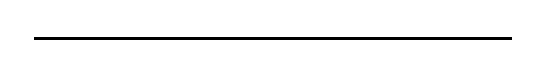
\begin{tikzpicture}
 		\draw[thick, black] (0.25*\textwidth, 0) -- (0.75*\textwidth, 0);
 		\node[rotate = 360 - 90, xshift = -0.6pt, yshift = 1pt] at (0.25*\textwidth,0){\decotwo};
 		\node[rotate = 90, xshift = -0.6pt, yshift = 1pt] at (0.75*\textwidth,0){\decotwo};
 	\end{tikzpicture}
 	\end{center}
 }
 
\newcommand{\signature}
{
	\begin{tikzpicture}[remember picture,overlay]
	\node[fill = YellowOrange!20!white] 
	at ([yshift = 1cm, xshift = -3cm]current page.south east) 
	{\fontsize{10pt}{0pt}{\itshape Kara.$\mathcal{A}$}};
	\end{tikzpicture}
}



\newtcolorbox[auto counter, number within= section]{definition}[1][]
 {
	 title = Definition~\thetcbcounter~ #1,
 	enhanced,
 	boxrule = 1pt,
 	fonttitle = \bf \color{black},
 	colback = white,
 	breakable,
        sharp corners,
 	% frame hidden,
        borderline west = {2pt}{0pt}{black},
	detach title,
	before upper = \tcbtitle \\,
	% attach title to upper = 
	% {
	% 	\\ \tld
	% },
	% after title = {\\},
	% before upper = \quad,
 	% attach boxed title to top left =
 	% {
 	% 	xshift = 0cm,
 	% },
 	% boxed title style =
 	% {
 	% 	colback = white,
 	% 	frame hidden
	% },
 }
 \newcommand{\lecday}[1][]
{
    \def\datee{#1}
    \fancyhead[L]{\datee}
}

\newtcolorbox[auto counter,number within= section]{theorem}[1][]
 {
	title = Theorem~\thetcbcounter~ #1,
 	enhanced,
 	boxrule = 1pt,
 	fonttitle = \bf \color{black},
 	colback = white,
 	breakable,
        sharp corners,
 	frame hidden,
        borderline west = {2pt}{0pt}{black},
	detach title,
	before upper = \tcbtitle \\,
 }

 \newtcolorbox[auto counter, number within = section]{proposition}[1][]
 {
	title = Proposition~\thetcbcounter #1,
 	enhanced,
 	boxrule = 1pt,
 	fonttitle = \bf \color{black},
	colback = white,
 	breakable,
        sharp corners,
 	frame hidden,
	detach title,
	before upper = \it \tcbtitle \quad ,
 }
 \newtcolorbox[auto counter, number within = section]{corollary}[1][]
 {
	title = Corollary~\thetcbcounter #1,
 	enhanced,
 	boxrule = 1pt,
 	fonttitle = \bf \color{black},
	colback = white,
 	breakable,
        sharp corners,
 	frame hidden,
	detach title,
	before upper = \it \tcbtitle \quad ,
 }
 \newtcolorbox{example}[1][]
 {
	title = Example, 
 	enhanced,
 	boxrule = 1pt,
 	fonttitle = \bf \color{black},
	colback = white,
 	breakable,
        sharp corners,
	detach title,
	before upper = \it \tcbtitle \quad ,
 }

 \newtcolorbox{remark}[1][]
 {
	title = Remark, 
 	enhanced,
 	boxrule = 1pt,
 	fonttitle = \bf \color{black},
	colback = white,
 	breakable,
        sharp corners,
	detach title,
	before upper =  \tcbtitle \it \quad ,
 }


% \newtcolorbox{proof}
% {
%      title = proof ,
% 	enhanced,
% 	boxrule = 1pt,
% 	fonttitle = \it \color{black},
%      colback = white,
% 	breakable,
%        sharp corners,
%      detach title,
%      before upper = \it \thetcbtitle \\ ,
% }





 \newcommand{\integral}[4]{\int\limits_{#1}^{#2} #4 d#3}
\newcommand{\limit}[3]{\lim\limits_{#1 \rightarrow #2} #3}
\newcommand{\strone}[2]{\left[ \begin{gathered}#1\\ #2\end{gathered} \right] }
\newcommand{\strtwo}[2]{\left\{ \begin{gathered}#1\\ #2\end{gathered} \right\} }
\newcommand{\strthree}[2]{\left\lfloor \begin{gathered}#1\\ #2\end{gathered} \right\rfloor }


\newcommand{\startbf}[1]{\text{\bfseries{#1}}}
\newcommand{\sett}[1]{\left\{ #1 \right\}}
\newcommand{\thesis}[1]{\left( #1 \right)}
\newcommand{\brkt}[1]{\left[ #1 \right]}
\newcommand{\floor}[1]{\left\lfloor #1 \right\rfloor}


\DeclareMathOperator{\img}{im} % Image
\DeclareMathOperator{\Img}{Im} % Image
\DeclareMathOperator{\coker}{coker} % Cokernel
\DeclareMathOperator{\Coker}{Coker} % Cokernel
\DeclareMathOperator{\Ker}{Ker} % Kernel
\DeclareMathOperator{\rank}{rank}
\DeclareMathOperator{\Spec}{Spec} % spectrum
\DeclareMathOperator{\Tr}{Tr} % trace
\DeclareMathOperator{\pr}{pr} % projection
\DeclareMathOperator{\ext}{ext} % extension
\DeclareMathOperator{\pred}{pred} % predecessor
\DeclareMathOperator{\dom}{dom} % domain
\DeclareMathOperator{\ran}{ran} % range
\DeclareMathOperator{\Hom}{Hom} % homomorphism
\DeclareMathOperator{\Mor}{Mor} % morphisms
\DeclareMathOperator{\End}{End} % endomorphism


\newcommand{\lm}{\ensuremath{\lambda}}
\newcommand{\eps}{\ensuremath{\epsilon}}
\newcommand{\veps}{\ensuremath{\varepsilon}}
\newcommand{\al}{\ensuremath{\alpha}}
\newcommand{\bb}{\ensuremath{\beta}}
\newcommand{\cc}{\ensuremath{\gamma}}
\newcommand{\dd}{\ensuremath{\delta}}
\newcommand{\DD}{\ensuremath{\Delta}}
\newcommand{\ff}{\ensuremath{\phi}}
\newcommand{\FF}{\ensuremath{\varphi}}

\newcommand{\RR}{\mathbb{R}}
\newcommand{\RO}{\mathcal{R}}
\newcommand{\EE}{\mathbb{E}}
\newcommand{\CC}{\mathbb{C}}
\newcommand{\RW}{\mathbb{R}^2}
\newcommand{\RT}{\mathbb{R}^3}
\newcommand{\RN}{\mathbb{R}^n}
\newcommand{\DS}{\mathcal{D}}

\newcommand{\KK}{\mathbb{K}}
\newcommand{\KW}{\mathbb{K}^2}
\newcommand{\KT}{\mathbb{K}^3}
\newcommand{\KN}{\mathbb{K}^n}

\newcommand{\NN}{\mathbb{N}}

\newcommand{\PS}{\mathcal{P}}
\newcommand{\AS}{\mathcal{E}}
\newcommand{\FS}{\mathcal{F}}
\newcommand{\LS}{\mathcal{L}}
\newcommand{\MS}{\mathcal{M}}


























\lecday[2025-03-06]

% \begin{document}

\section{An important isomorphism isometric}

Let $E,F$ and $G $ be three N.V.S over the same 
field $\KK = \RR  \text{ or }  \CC  $, then there exist
a natural transformation from 
$\mathcal{L}(E, \mathcal{L} (F,G)) $  to 
$\mathcal{L} \left( E,F ;G \right) $, which is defined
by 
\[
\begin{array}{cccc}
      i : &  \mathcal{L} 
	  \left( E, \mathcal{L} 
\left( F,G \right)\right)& \longrightarrow & 
\mathcal{L} \left( F,F ; G \right)\\

           &  f  & \longmapsto     & 
	   i \left( f \right) : 
	   \vspace{2pt}
	   \begin{array}{cccc}
	            &  
		  E \times F & \longrightarrow & 
		  G \\
	              & (x,y)     & \longmapsto     &
		      i(f) (x,y) = 
		      f(x)  f(y) \\ 
	   \end{array}
	   \\ 
\end{array}
\]
Its easy to show that its well defined, linear and
bijective with $i^{-1} $ give :

\[
\begin{array}{cccc}
      i^{-1} : &  
	       \mathcal{L} (E,F;G) & \longrightarrow & 
	       \mathcal{L} \left( E, \mathcal{L} (F,G)  \right)\\
           &  g  & \longmapsto     & i^{-1}(g)  : 
	   \begin{array}{cccc}
	           &  E   & \longrightarrow &  \mathcal{L}
		   (F,G) \\
	              &    x& \longmapsto     & i^{-1}(g) (x)   
	   \end{array} 
	   : 
	   \begin{array}{cccc}
	           &  F  & \longrightarrow &  G \\
	   
	              &   y& \longmapsto     & 
		      i^{-1}(g) (x) (y) = g(x,y)  \\
	   \end{array}
\end{array}
\]
now let us show that $i $ is an isometry, with respect to the natural
norms defined on $\mathcal{L} (E,F;G)  $  and 
$\mathcal{L} (E,\mathcal{L} (F,G) )  $, for all 
$f \in  \mathcal{L} (E, \mathcal{L} (F,G) )  $, we have 
\begin{align*}
\| i(f)  \| _{ \mathcal{L} (E,F;G) } = 
\sup_{
	\small
	\begin{gathered}  
		x \in  E \backslash {0_{E}}\\  
		y \in  F \backslash {0_{F}}
	\end{gathered}
	\normalfont
} 
\frac{\| i(f) (x,y)  \| _{G}}{
\| x \| _{E} \| y \| _{F}} &= 
\sup_{
	\small
	\begin{gathered}  
		x \in E \backslash {0_{E}}\\ 
		x \in F \backslash {0_{F}}\\ 
	\end{gathered}
	\normalfont
} 
\frac{\| f(x) (y)  \| _{G}}{
\| x \| _{E} \| y \| _{F}}
\\
			   &= 
\sup_{x \in E \backslash \left\{ 0_{E} \right\}}  
\frac{1}{\| x \| _{E}}  
\sup_{y \in  F \backslash \left\{ 0_{F} \right\}}  
\frac{\| f(x,y)  \| _{G}}{
\| y \| _{F}} \\
&= \sup_{x \in E \backslash \left\{ 0_{E} \right\}}  
\frac{1}{\| x \| _{E}} 
\| f(x) _{\mathcal{L} (F,G) } \|  \\
&= 
\| f \| _{\mathcal{L} \left( E,\mathcal{L} (F,G)  \right)}
\end{align*}
that is $i $ is an isometry, because
of the isomorphism isometric 
$i $ between $\mathcal{L} (E, \mathcal{L} (F,G) )  $ 
and $\mathcal{L} (E,F;G)  $, we often identify 
$\mathcal{L} (E,\mathcal{L} (F,G) )  $ to 
$\mathcal{L} (E,F;G)  $, This is used 
in particular in differential calculus on N.V.S 
(for defining second derivative)
\section{An introduction to differential calculus in N.V.S}
Let $E $ and $F $ be two N.V.S over the a same
field $\KK = \RR  $ or $\CC  $, and let $U $ be an open 
subset of $E $ and $a \in U $. Finally, let 
$ f : U \longrightarrow F $ be a map
\begin{definition}[]
We say that $f $ is differentiable at $a $ if there exist
$g \in  \mathcal{L} (E,F)$ so that we have
in the neighborhood of $a$
\[
\| f(x) -f(a)  - g(x-a)   \| _{F} = 
o \left( \| x-a \|_{E}  \right) 
\]
\end{definition}
\begin{remark}[]
\begin{enumerate}[(1)]
\item  If $f $ is differentiable at $a $ then 
	$f $ is continuous at $a $. Indeed, by letting
	$x \rightarrow a $, we obtain since ( $g $ is continuous
	at $0_{E} $ ), that $\lim_{x \to a} f(x) = f(a)  $, 
	showing that $f $ is continuous at $a $.
\item  If $f $ is idfferentiable at $a $ then the continuous
	linear mapping $g $ is unique.
\end{enumerate}
\end{remark}
\begin{proof}
	Let $g_1,g_2 \in \mathcal{L} (E,F)  $, each of them
	satisfies 
	\begin{align*}
		\| f(x) -f(a) - g_1(x-a)  \| _{F} &=
	o \left( \| x-a \|_{E}  \right)
	\\
		\| f(x) -f(a) - g_2(x-a)  \| _{F} &= 
	o \left( \| x-a \|_{E}  \right)
	\end{align*}
	when $x $ is in the neighborhood of $a$, 
	so for all $h \in E $ ( in the neighborhood of 
	$0_{E} $ , we have 
	\begin{align*}
		\| (g_1-g_2) (h)  \| _{F} &= 
		\| g_1(h) - g_2(h)  \| _{F} \\
	  &=  
	  \| 
	  \left( f(a+h) -f(a) -g_2(h)  \right) - 
	  \left( f(a+h) -f(a) -g_1(h)  \right)
	  \|  \\
	  & \leq 
	  \underbrace{
	  \| f(a+h) -f(a) -g_2(h)  \| _{F}
	  }_{o(\| h \| _{E}) }  + 
	  \underbrace{
	  \| f(a+h) -f(a) -g_1(h)  \| _{F}
	  }_{o(\| h \| _{E})  }  = o
	  (\| h \| _{E}) 
	\end{align*}
	Thus $\| (g_1 - g_2) (h)  \| _{F} = o(\| h \| _{E})  $,
	in other words 
	\[
	\lim_{\| h \| _{E} \to 0} 
	\frac{\| (g_1-g_2) (h)  \| _{F}}{
		\| h \| _{E}
	} = 0
	\]
	now let $x \in  E \backslash \left\{ 0_{E} \right\} $  
	be arbitrary, by taking $h = \veps x  $ and
	$(\veps  \rightarrow^{> } 0)  $, we get 
	\[
	\lim_{\veps  \to ^{> } 0} 
	\frac{
	\| (g_1 - g_2) (\veps x)  \| _{F}
	}{
		\| \veps x \| _{E}
	} = 
	0
	\]
	thus we see 
	\[
		\frac{	
	\| (g_1 - g_2)(x)   \|_{F}
		}{
			\| x \| _{E}
		} = 0
	\]
	thus we see that 
	\[
	g_1(x)  = g_2(x)  \quad 
	\left( \forall  x \in  E \backslash \left\{ 0_{E}
	\right\} \right)
	\]
	which remains true for $x = 0_{E} $, hence
	$g_1 (x) = g_2(x)  $  for all $x \in E $, therefore
	$g_1 = g_2 $, by the uniqueness of $g $ is then
	proved.
\end{proof}
\begin{definition}[]
	If $f $ is differentiable 
	at $a $ then the continuous linear mapping $g $ 
	satisfying
	\[
	\| f(x) -f(a) - g(x-a)  \|_{F}  = 
	o(\| x-a \|_{E} ) 
	\]
	is called
	\begin{center}
		\it
		The derivative of $f $ at $a $, and it's 
		denoted $f'(a)  $ 
		\normalfont
	\end{center}
\end{definition}
\section{Relationship with the classical case 
	\texorpdfstring{$ E = F = \RR $}{E=F=R}
}
If $E = F = \RR $, and $U $ is an open subset of $\RR  $,
$ f : U \longrightarrow \RR $, and $a \in U $ then the classical
definition of the differentiability states that 
\begin{center}
	\it
	$f $ is differentiable at $a $ if 
	$\lim_{x \to a} \frac{f(x) -f(a) }{x-a} $  
	exsits (i.e. $ \in \RR  $)
	\normalfont
\end{center}
So if its the case and we let 
\[
l := 
\lim_{x \to a} 
\frac{f(x) - f(a)  }{ x-a}
\]
we desire that 
\[
\lim_{x \to a}
\left( 
	\frac{f(x) -f(a) }{x-a} - l
\right) = 0
\]
that is 
\[
\lim_{x \to a} 
\frac{f(x) -f(a) -l(x-a) }{x-a} = 0
\]
therefore we see
\[
\left| f(x) -f(a) -l(x-a)  \right| = o (\left| x-a \right|)  
\quad  \text{ when } x \rightarrow a
\]
so hence 
\[
\begin{array}{cccc}
      g : &  \RR   & \longrightarrow & \RR  \\
           &  x  & \longmapsto     & lx \\ 
          \in  \mathcal{L} (\RR ,\RR ) 
\end{array}
\]
satisfies, so in the sense of Definition $2$, 
$f $ is differnetiable at $a $ and 
\[
f'(a)  = 
\left[ 
	\begin{array}{cccc}
	        & \RR     & \longrightarrow &  \RR \\
	
	           &    x& \longmapsto     &  lx \\ 
	\end{array}
\right]
\]
By identifying the homothety of center
$0 $ and ratio $l$ to $l $, we obtain the equivalence
between the classical case 
$(E=F=\RR )  $, and the general case on N.V.S
\[
\begin{array}{cccc}
       : &  \RR   & \longrightarrow & 
       \mathcal{L} (\RR ,\RR ) \\

           &  l  & \longmapsto     & \mathcal{H}(0,l):
	   \begin{array}{cccc}
	             &  \RR    & \longrightarrow &  \RR  \\
	   
	              & x    & \longmapsto     &  lx \\
	   \end{array}
\end{array}
\]
is an isomorphism isometric. \\
In fact, we identify $\mathcal{L} (\RR ,\RR )  $ 
with $\RR  $.
\begin{definition}[]
We say that $f $ is differentiable in $U $, if its differnetiable
at every point of $U $. 
\begin{itemize}
\item If $f $ is differentiable in $U $ then it's
	derivative is the map $f' $ defined by : 
	\[
	\begin{array}{cccc}
	      f' : &  U  & \longrightarrow & 
	      \mathcal{L} (E,F) \\
	           &  a  & \longmapsto     & f'(a)  \\ 
	\end{array}
	\]
	In the particular case $E = \RR  $, 
	we can identify $\mathcal{L} (E,F) = 
	\mathcal{L} (\RR ,F)$ to $F $, so we obtain
	$ f' : U \longrightarrow F $ as in the classical
	case $E = F = \RR  $.
\end{itemize}
\end{definition}
\section{The Second Derivative}
Let $E $ and $F $ be two N.V.S, and $U $ be an open
subset of $E $, and $ f : U \longrightarrow F $ suppose that 
$f $ is differentiable in $U $ and let 
$ f' : U \longrightarrow \mathcal{L} (E,F)  $ be it's 
derivative so we can ask if $f' $ is differentiable in $U$ 
\begin{definition}[]
We say that $f $ is twice differentiable 
at $a  \in U$ if $f'  $ is differentiable at $a $. In this
case we denote $f''(a)   $ the derivative of $f' $  at
$a $, so 
\[
f''(a) \in  
\mathcal{L} (E, \mathcal{L} (E,F) ) 
\]
called the second derivative of $f $ at $a$. 
\end{definition}
\begin{definition}[]
We say that $f $ is twice differentiable in $U $ if 
its twice differentiable at every point 
of $U$. In such a case, the second derivative of $f$ is the 
map.
\[
\begin{array}{cccc}
      f'' : &  U  & \longrightarrow & 
      \mathcal{L} (E, 
      \mathcal{L} (E,F) ) \\
           &   a & \longmapsto     & f''(a)  \\
\end{array}
\]
\end{definition}
Then we often consider $f''( a) (a \in U)   $, as
an element of $\mathcal{L} (E,E;F)  $ that is 
$f''(a)  $ is a continuous bilinear map from 
$E \times E$ to $F$.
% \end{document}
